\documentclass[a4paper,12pt]{article}
\usepackage{amsmath,amsfonts,amssymb,fancyhdr,graphicx,mathdots,cancel,sidecap,floatrow,cite}
\usepackage{etoolbox}
\patchcmd{\thebibliography}{\section*{\refname}}{}{}{}
\def\mb#1{$\mathbf{#1}$}
\def\hnorm#1{\vert\vert #1 \vert\vert_{H^1(\Omega)}}
\def\lnorm#1{\vert\vert #1 \vert\vert_{L^2(\Omega)}}
\def\unorm#1{\vert\vert #1 \vert\vert_{U}}
\def\vnorm#1{\vert\vert #1 \vert\vert_{V}}
\def\norm#1{\vert\vert #1 \vert\vert}
\def\abs#1{\vert #1 \vert}
\def\xh{\hat{x}}
\addtolength{\evensidemargin}{-2cm}
\addtolength{\oddsidemargin}{-2cm}
\addtolength{\textwidth}{3cm}
\addtolength{\textheight}{0cm}
\fancyhead[L]{Progress Report}
\fancyhead[R]{Jonathan deWerd}
\begin{document}
\section{Background}
\subsection{PNA}
Artificial nucleic acids hold the promise of retaining the antisense recognition property of DNA and RNA while allowing for enhanced physical properties such as increased cellular uptake (Zhou, 2003), decreased nuclease degradation rate (Singh, 1998), and larger free energies of binding (Kurreck, 2003) as compared to their natural counterparts.

\begin{figure}[H]
	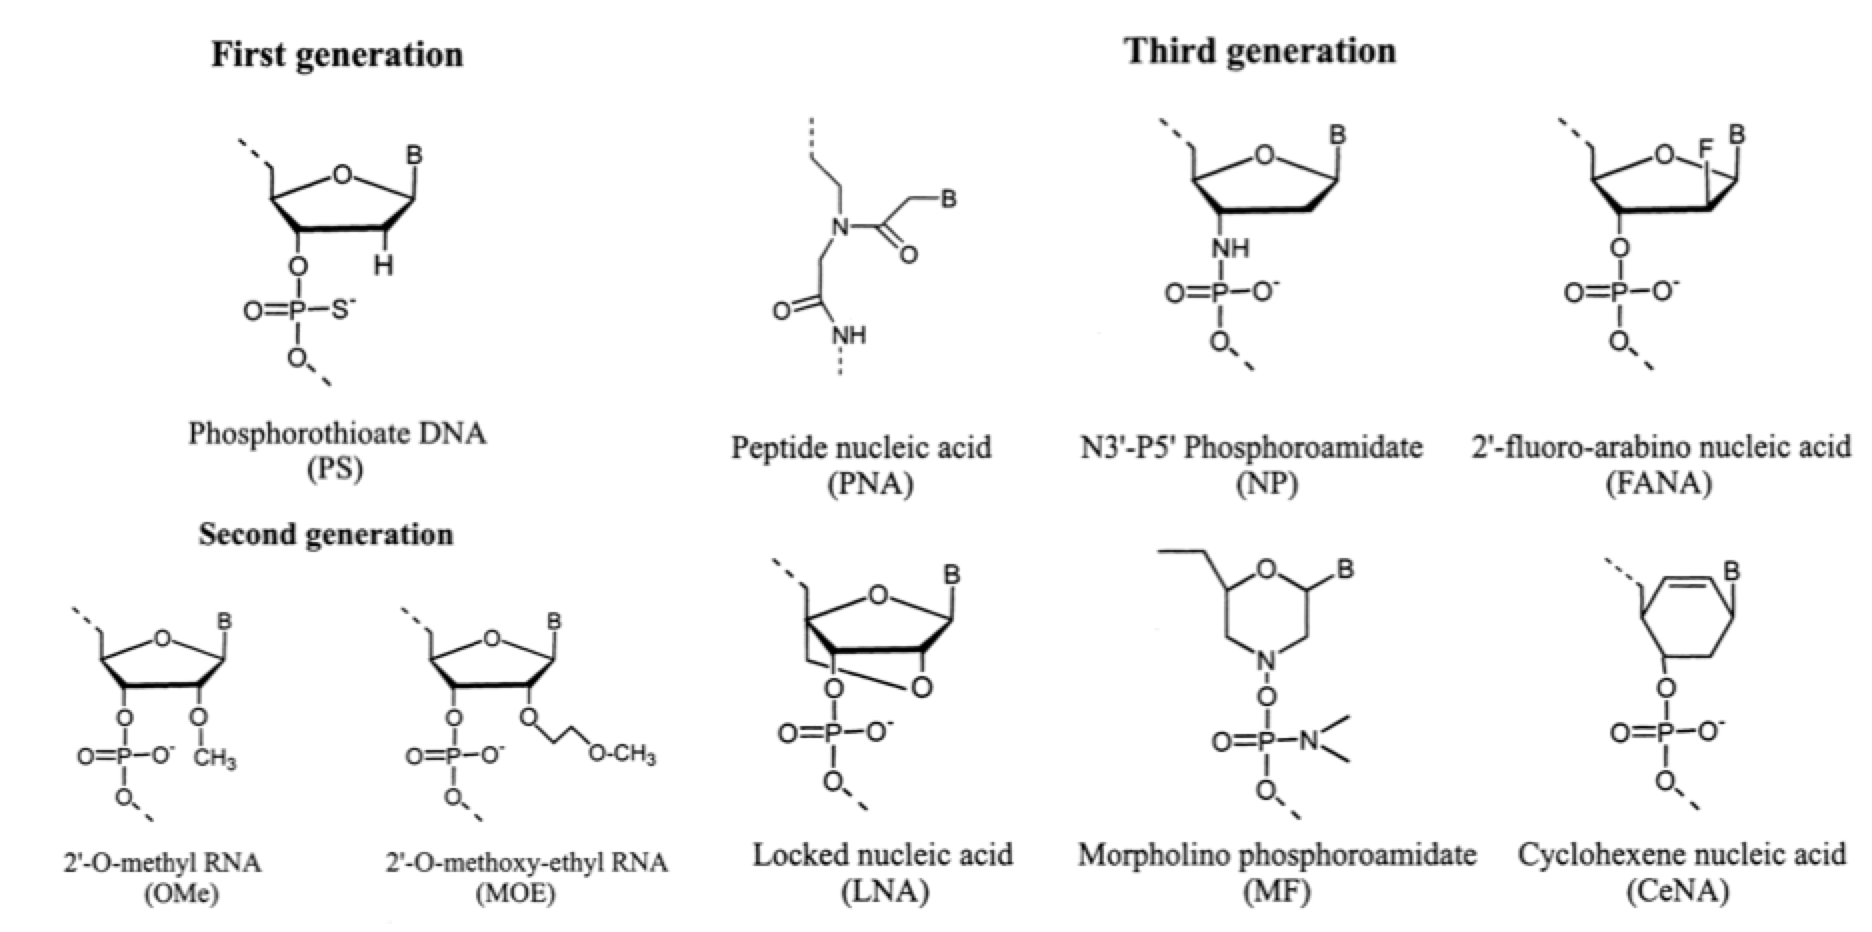
\includegraphics[height=2.5in]{generations.png}
	\caption{\it The three ``generations'' of artificial nucleic acids, according to Kurreck, 2003.}
\end{figure}

``PNA,'' the artificial amino acid based on a peptide as opposed to phosphoribose backbone, is known for pre-arranging into low-entropy helices in its single-stranded form (Sforza, 1999). This property allows it to form PNA-DNA and PNA-RNA complexes with $\Delta G^0_{37}$ energies approximately 150\% of those typical of DNA-DNA or RNA-RNA complexes (e.g. Griffin, 1998 reports a free energy of $1.5\frac{kcal}{mol\cdot bp}$ for $AA_{PNA}-TT_{DNA}$ while the 1998 SantaLucia meta-analysis reports a free energy of $\sim1.0\frac{kcal}{mol\cdot bp}$ for $AA_{DNA}-TT_{DNA}$). For a 10-mer, this translates to a $10^\circ$C-$20^\circ$C difference in melting temperature $T_m$. In any case, the increased thermodynamic stability suggests that applications such as antisense tagging of ribosomes and other RNAzymes for single-molecule studies could greatly benefit from using PNA. These studies currently use DNA oligomers but are limited by the thermodynamic stability of short DNA oligomers and the inflexibility of long DNA oligomers (Marshall, 2008), making $\gamma$PNA a tempting alternative. 

\subsection{Strand Invasion}
While the thermodynamics of PNA-RNA complexes are promising, there have been significant kinetic challenges involved with persuading PNA to invade double-stranded DNA and RNA helices without a denature/anneal step. In particular, arbitrary PNA sequences generally {\it do not} invade DNA and RNA helices at room temperature (He, 2009). PNA was originally designed to bind helices using Hoogsteen-pairing in the major groove; Watson-Crick pairing was discovered by accident  and many alternative strategies of achieving Watson-Crick pairing were subsequently developed (Kaihatsu, 2003):
\begin{enumerate}
\item {\bf Homopyrimidine PNA:} the original PNA paper used PNA strands composed entirely of pyrimidine bases on account of the fact that homopyrimidine and homopurine DNA oligomers are typically far better than their mixed-base counterparts at forming a triplex by binding to the major groove of a DNA helix using Hoogsteen pairing. However, they discovered that PNAs composed entirely of pyrimidine bases were able to invade complementary regions of target helices in order to bind them in a Watson-Crick fashion (Peffer, 1993). A second strand of PNA subsequently bound the same region on the Hoogsteen edge to form a ``PNA$_2$-DNA'' complex (Wittung, 1996).
\item {\bf Homopurine PNA:} similar to homopyrimidine PNA.
\item {\bf bis-PNA:} covalently linking two strands of homopyrimidine PNA improves invasion kinetics and decreases pH and salt dependence so that binding can happen under physiological conditions (Egholm, 1994).
\item {\bf cationic-PNA:} inserting positively charged amino acids (typically lysine) into the linker of bis-PNA gives them a 100-fold (Kaihatsu, 2002) to 1000-fold (Griffith, 1995) improvement in EC$_{50}$. Plain PNA improved by 4x (Griffith, 1995).
\item {\bf pc-PNA:} pseudocomplementary PNA uses nonstandard basepairs to dissuade PNA-PNA binding (but not DNA-PNA or RNA-PNA binding) so that complementary PNA oligos may be used. This significantly relaxes the homopyrimidine constraint ($\sim$80\% of sequences can be targeted with this strategy according to Lohse, 1999).
\item {\bf Supercoiled DNA Target:} genomic and plasmid DNA are maintained in an underwound state to facilitate strand separation (e.g. by polymerases). This allows PNA to target mixed-base sites in genomic and plasmid DNA (Zhang, 2000).
\item {\bf TailClamp-PNA:} a 6*2-bp ``tail clamp'' (toehold) of homopyrimidine base pairs suffices to enable strand invasion (Kaihatsu, 2003).
\item {\bf Intercalator-PNA:} conjugating a PNA with the intercalator 9-aminoacridine decreases EC$_{50}$ values by a factor of 100-150 for cationic-PNA (Bentin, 2003).
\item {\bf $\gamma$PNA:} allows mixed-sequence PNA oligomers to invade DNA helices.
\item {\bf Low [Na$^+$]+[Mg$^+$]:} Due to its anionic backbone, the stability of DNA and RNA secondary structure is heavily dependent on cation concentration. Reducing the cation concentration greatly facilitates PNA binding (Peffer, 1993).
\end{enumerate}
\begin{figure}[H]
\makebox{
	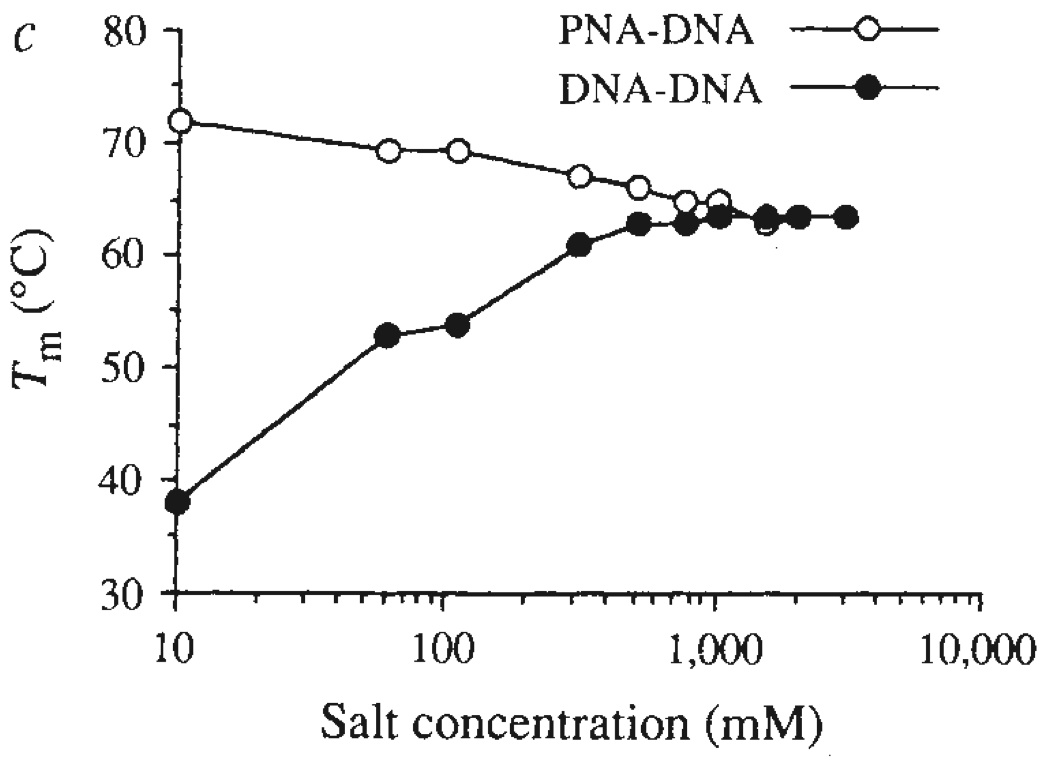
\includegraphics[height=2in]{salt.png}
	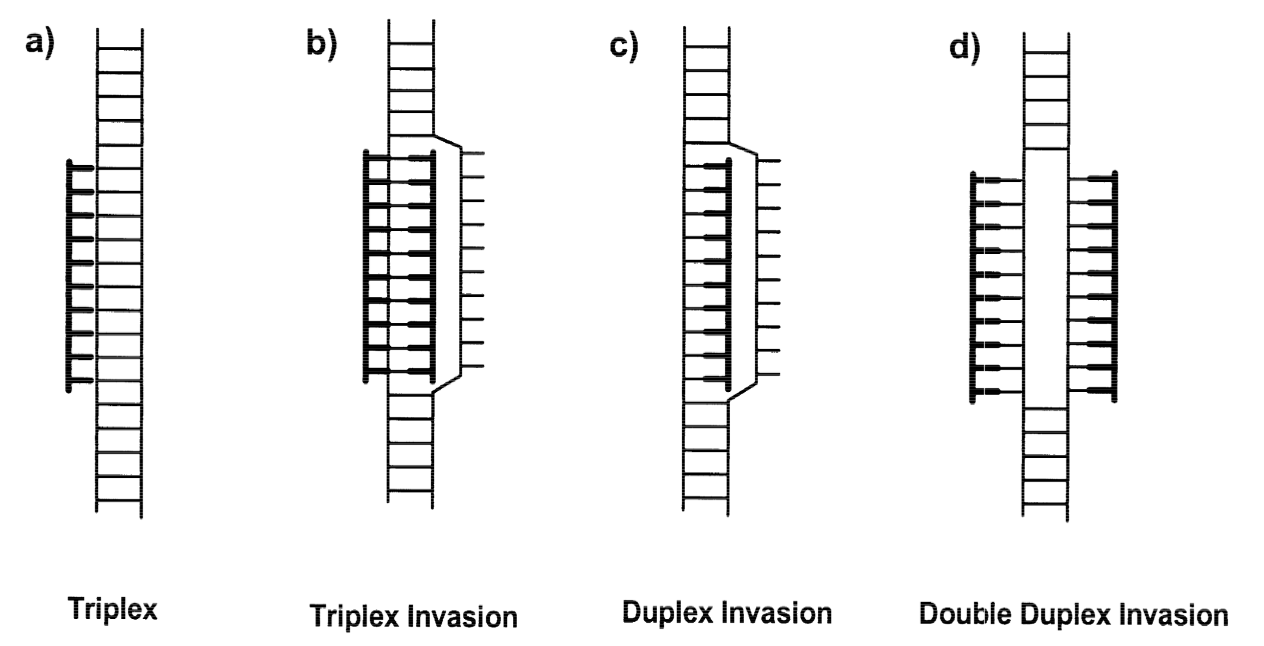
\includegraphics[height=2in]{bindingmodes.png}
}
	\caption{\it Left: salt dependence of duplex $T_m$s (Egholm, 1993). Right: binding terminology (Koppelhus, 2003).}
	\label{invasionmodes}
\end{figure}

\subsection{Particularly Relevant Previous Work}
\begin{enumerate}
\item {\bf Peffer, 1993:} Notes an abundance of evidence that strand invasion is rate-limited by ``DNA Breathing'' (thermodynamic fluctuations temporarily opening the helix). This explains why homopyrimidine PNA is particularly good at strand invasion: the triplex transition state is far more stable than it would be for a mixed sequence, even if the product thermodynamics are similar. The strength of THz radiation required to athermally induce ``breather'' modes in nucleic acids (i.e. accelerate PNA invasion kinetics) is far greater than what can be achieved in lab (Swanson, 2010).
\item {\bf Good, 1998:} Cationic homopyrimidine bis-PNA is able to inhibit in-vitro bacterial translation, but cationic mixed-sequence PNA is not. 
\item {\bf Dias, 2002:} Plain mixed-sequence PNA is able to bind mRNA hairpins given 4-6bp toeholds in unpaired regions. At 1$\mu M$, 13-mers, 12-mers, and 11-mers achieved $80\%, 40\%,$ and $30\%$ translation inhibition (pH 7, 100mM KCl). Significant pH and salt dependence was observed.
\end{enumerate}

\subsection{Implications for Current Work}
\begin{itemize}
\item Ion concentrations are crucial for the free energy of invasion ($\Delta G_{pna-dna}-\Delta G_{dna-dna}$) and invasion kinetics (RNA ``breathing'') even if they are not significant for $\Delta G_{pna-dna}-\Delta G_{rand.coil.}$ (free energy of binding). We now have two ``knobs'' by which to adjust invasion kinetics/thermodynamics: PNA concentration and salt concentration. The latter is unique in that it has the potential to affect kinetics, which are often a limiting factor, in a superlinear fashion.
\item pH differences as small as pH7$\rightarrow$pH8 or ph7$\rightarrow$pH6 and PNA concentration differences can select between invasion modes (Figure \ref{invasionmodes}) (Dias, 2002). This might lead to an atypical dose-dependency for PNA binding.
\item While adjusting salt concentrations suffices to ensure binding in-vitro, in-vivo studies could probably use a recommender system to inform the choice between types of PNA (perhaps a kinetic relation could be derived from the PBD ``breather'' model used in the THz-radiation literature).
\end{itemize}


\section{Experiments}
\subsection{Previous work: SHAPE}
The Selective 2'-Hydroxyl Acylation Protection from Exoribonuclease (SHAPE) assay differs from previous RNA footprinting assays in that it produces information on local nucleotide flexibility rather than reporting on the presence of a base pair (e.g. as DMS footprinting would) or the solvent accessibility (as hydroxy-radical footprinting would) (Weeks, 2010). This makes it particularly well suited to inferring thermodynamic information which cannot be inferred from the secondary structure or crystal structure alone (Low, 2010).
\begin{figure}[H]
	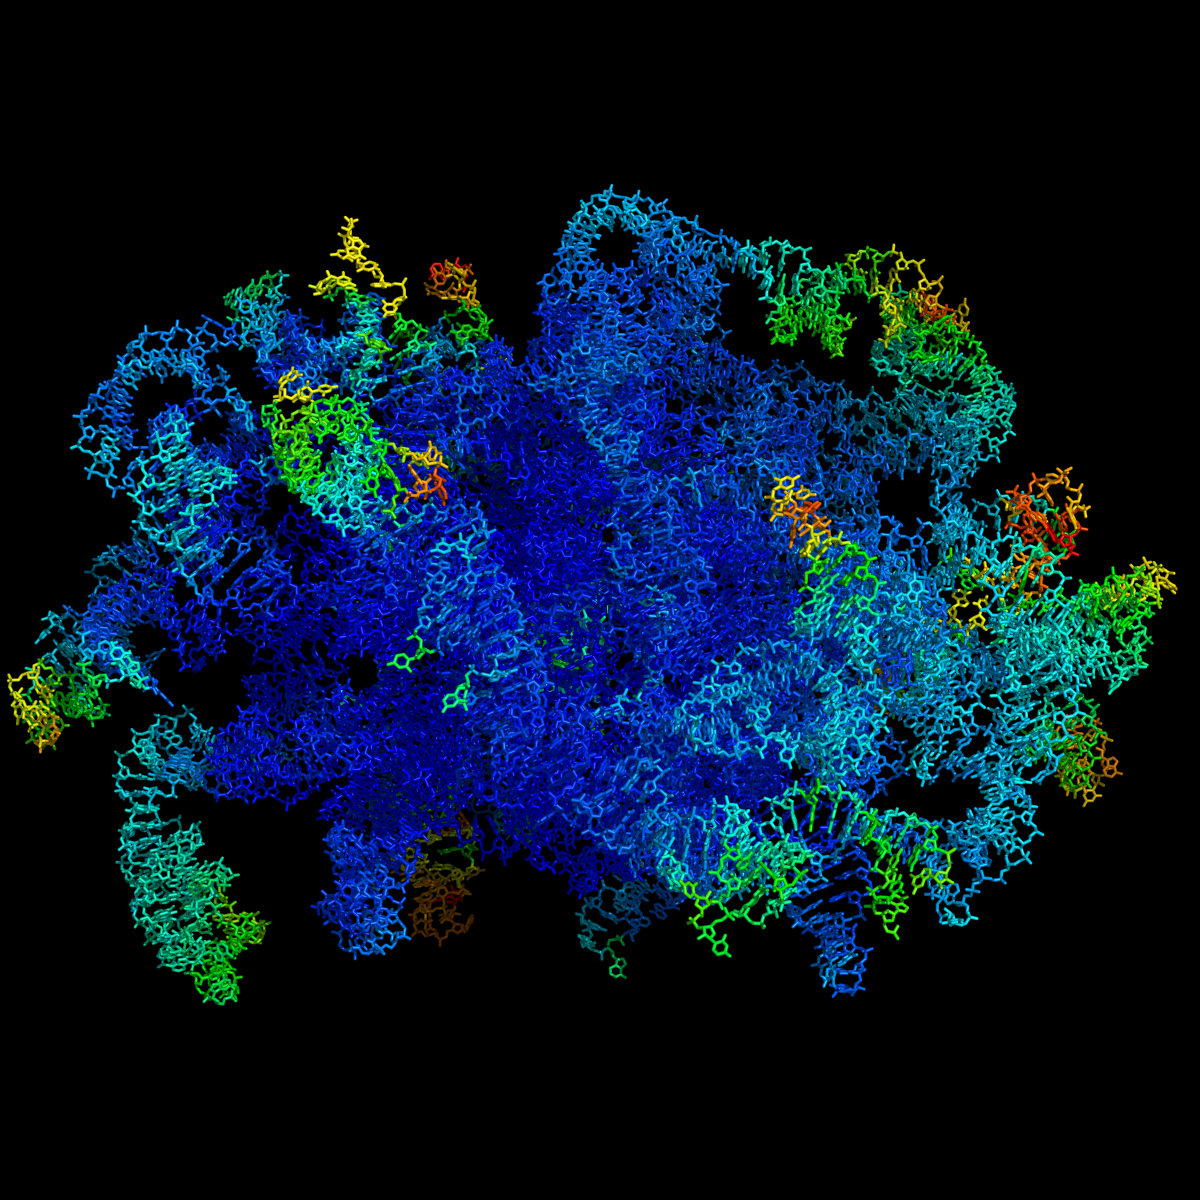
\includegraphics[height=2.5in]{beta_heatmap.png}
	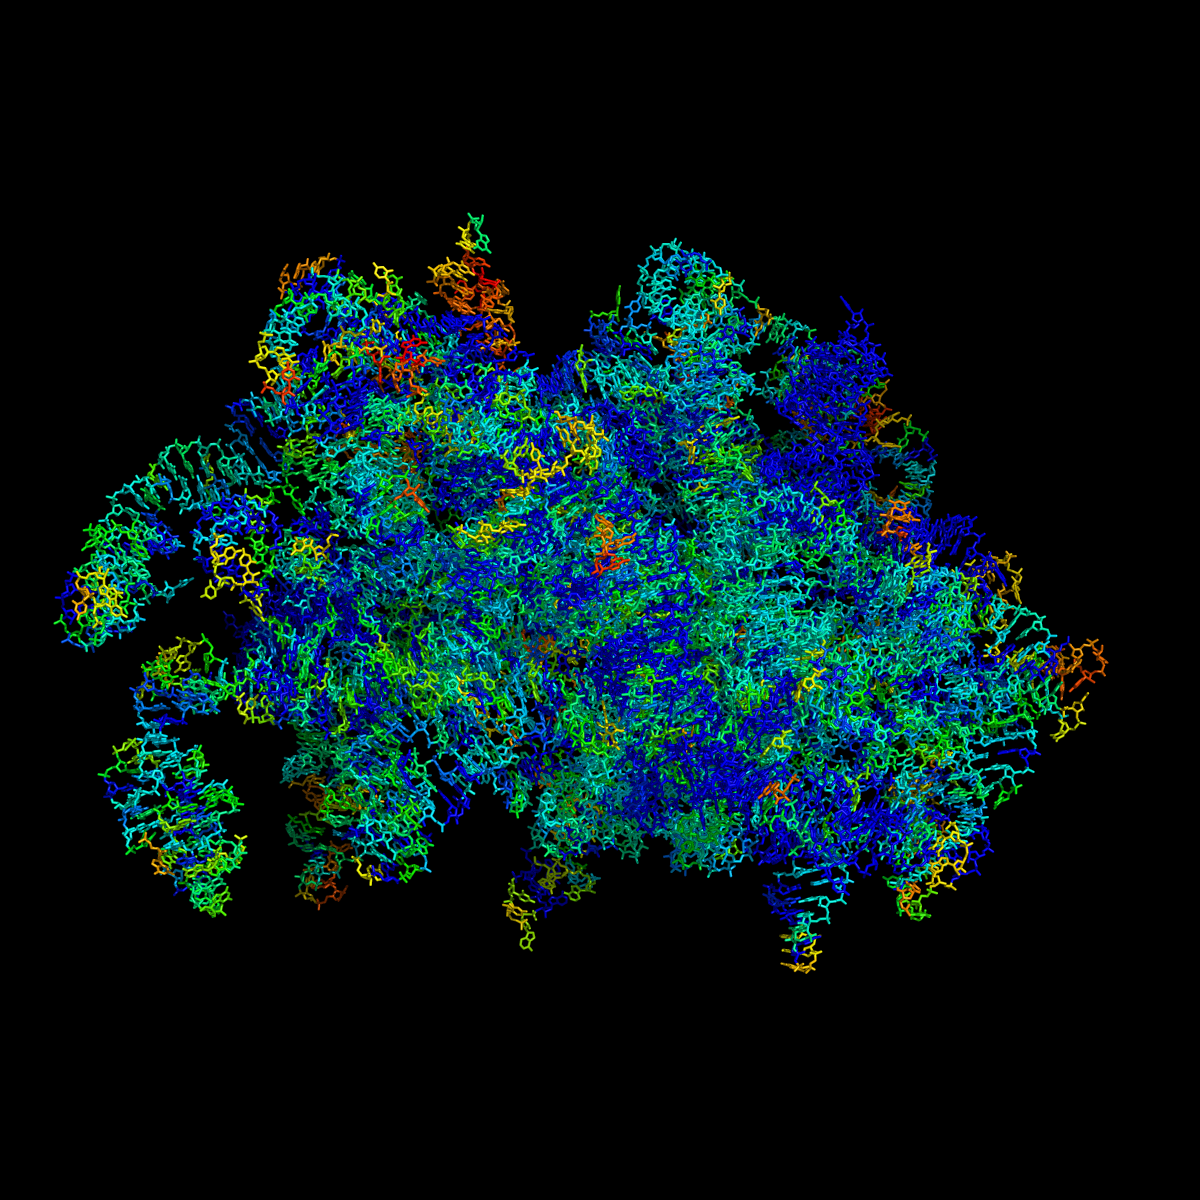
\includegraphics[height=2.5in]{dinman_heatmap.png}
	\caption{\it Left: beta factors (ensemble flexibility in the crystal structure) from the 3U5H Cerevisiae large subunit (Ben-Shem, 2011). Right: logarithmic SHAPE reactivity of the solvated Cerevisiae large subunit (unpublished data, Dinman group).}
\end{figure}
Although the SHAPE experiment produced noisier data than the crystallography experiment, it is important to keep in mind that 1. the SHAPE data is more relevant to physiological conditions (temperature, solvation, ion concentration) and 2. the SHAPE data still follows the same broad trend of high reactivity on exposed hairpins and low reactivity in the relatively stable ribosomal core. This trend is exaggerated in the crystallography data to an extent that would be puzzling if it came from a SHAPE reaction: the core of the ribosome should not be 

\subsection{Previous work: Translation Inhibition}

\subsection{Current work: Translation Inhibition}
\subsection{Current work: Molecular Dynamics}



\section{Discussion \& Analysis}
\section{Goals}


\end{document}